\section{Noen enkle forord} \label{sec: forord}

Dette er kun noen enkle forord. 
Vi skal skrive om SOFiSTiK og \LaTeX!

Nå skal jeg teste hvordan genereringen av bilder vha. Python fungerer. Jeg har da laget et sinus-plot i Python,
lagret den til valgt mappe, og skal nå forsøke å printe den her vha. \LaTeX. Her er bildet, en liten test først selvfølgelig:

\begin{figure}[h]
    \centering
    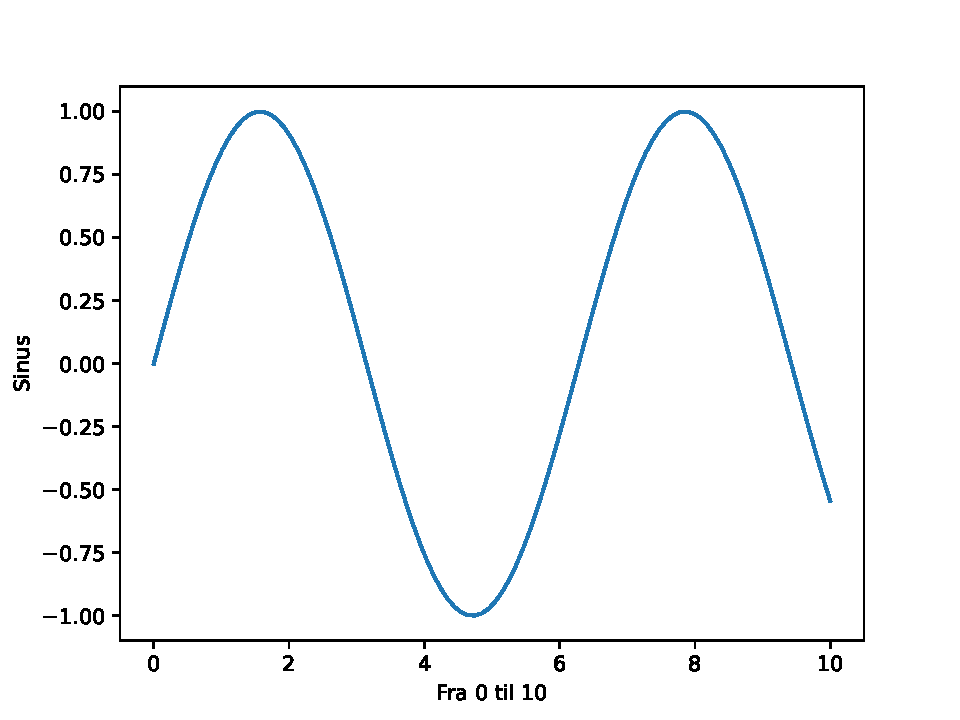
\includegraphics[width=0.5\textwidth]{0 FIGURER/sinus}
    \caption{Figur 1}
    \label{fig:figure}
\end{figure}


\begin{figure}[h!]
    \centering
    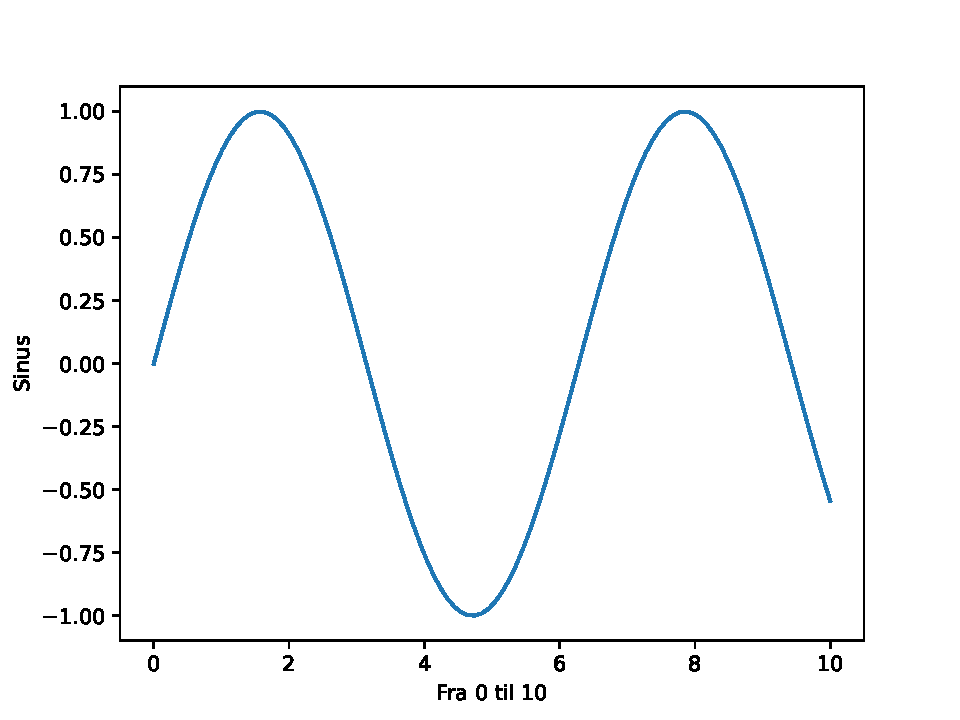
\includegraphics[width=0.5\textwidth]{0 FIGURER/sinus.pdf}
    \caption{Hei}
    \label{fig:hei}
\end{figure} 

\vspace{2mm}